\documentclass[11pt]{report}
\usepackage{multicol,lipsum,microtype}
\usepackage[table, xcdraw,dvipsnames]{xcolor}
\usepackage[backend=biber]{biblatex}
\addbibresource{bib/main.bib}
\usepackage{vub}
\usepackage{listings}
\usepackage{lstautogobble}  % Fix relative indenting
\usepackage{xargs}
\usepackage{float}
\usepackage{tikz}
\usepackage{bytefield}
\usepackage{pgf-umlsd}
\usepackage{pgfplots}
\pgfplotsset{compat=1.16}
\usepgfplotslibrary{statistics}
\usepgfplotslibrary{groupplots}
\usepackage{caption}
\usepackage{subcaption}
\usepackage{acronym}
\usepackage{mathtools}
\usepackage{amssymb}
\usepackage{amsmath}
\usepackage{zi4}            % Nice font
\usepackage{booktabs}
\usepackage{multirow}
\usepackage[toc,page]{appendix}

\definecolor{bluekeywords}{rgb}{0.13, 0.13, 1}
\definecolor{greencomments}{rgb}{0, 0.5, 0}
\definecolor{redstrings}{rgb}{0.9, 0, 0}
\definecolor{graynumbers}{rgb}{0.5, 0.5, 0.5}

\usepackage[colorinlistoftodos,prependcaption,textsize=tiny]{todonotes}
\newcommandx{\unsure}[2][1=]{\todo[linecolor=red,backgroundcolor=red!25,bordercolor=red,#1]{#2}}
\newcommandx{\change}[2][1=]{\todo[linecolor=blue,backgroundcolor=blue!25,bordercolor=blue,#1]{#2}}
\newcommandx{\info}[2][1=]{\todo[linecolor=OliveGreen,backgroundcolor=OliveGreen!25,bordercolor=OliveGreen,#1]{#2}}
\newcommandx{\improvement}[2][1=]{\todo[linecolor=Plum,backgroundcolor=Plum!25,bordercolor=Plum,#1]{#2}}
\newcommandx{\thiswillnotshow}[2][1=]{\todo[disable,#1]{#2}}

% \usetikzlibrary{external}
% \tikzexternalize[prefix=tikz/]
% \usepackage[a4paper,landscape,hmargin={1cm,1cm}]{geometry}
\usepackage{tikz-timing}[2014/10/29]
\usetikztiminglibrary[rising arrows]{clockarrows}
\usetikzlibrary{fit}
\usetikzlibrary{calc}
\usetikzlibrary{quotes}
\usetikzlibrary{positioning}
\usetikzlibrary{arrows,automata}
\usetikzlibrary{backgrounds,calc,shadings,shadows}
\usepackage{circuitikz}
\usetikzlibrary{shapes,decorations.pathreplacing}

\tikzstyle{bag} = [align=center]

\makeatletter
\pgfkeys{/pgf/.cd,
  parallelepiped offset x/.initial=2mm,
  parallelepiped offset y/.initial=2mm
}
\pgfdeclareshape{parallelepiped}
{
  \inheritsavedanchors[from=rectangle] % this is nearly a rectangle
  \inheritanchorborder[from=rectangle]
  \inheritanchor[from=rectangle]{north}
  \inheritanchor[from=rectangle]{north west}
  \inheritanchor[from=rectangle]{north east}
  \inheritanchor[from=rectangle]{center}
  \inheritanchor[from=rectangle]{west}
  \inheritanchor[from=rectangle]{east}
  \inheritanchor[from=rectangle]{mid}
  \inheritanchor[from=rectangle]{mid west}
  \inheritanchor[from=rectangle]{mid east}
  \inheritanchor[from=rectangle]{base}
  \inheritanchor[from=rectangle]{base west}
  \inheritanchor[from=rectangle]{base east}
  \inheritanchor[from=rectangle]{south}
  \inheritanchor[from=rectangle]{south west}
  \inheritanchor[from=rectangle]{south east}
  \backgroundpath{
    % store lower right in xa/ya and upper right in xb/yb
    \southwest \pgf@xa=\pgf@x \pgf@ya=\pgf@y
    \northeast \pgf@xb=\pgf@x \pgf@yb=\pgf@y
    \pgfmathsetlength\pgfutil@tempdima{\pgfkeysvalueof{/pgf/parallelepiped
      offset x}}
    \pgfmathsetlength\pgfutil@tempdimb{\pgfkeysvalueof{/pgf/parallelepiped
      offset y}}
    \def\ppd@offset{\pgfpoint{\pgfutil@tempdima}{\pgfutil@tempdimb}}
    \pgfpathmoveto{\pgfqpoint{\pgf@xa}{\pgf@ya}}
    \pgfpathlineto{\pgfqpoint{\pgf@xb}{\pgf@ya}}
    \pgfpathlineto{\pgfqpoint{\pgf@xb}{\pgf@yb}}
    \pgfpathlineto{\pgfqpoint{\pgf@xa}{\pgf@yb}}
    \pgfpathclose
    \pgfpathmoveto{\pgfqpoint{\pgf@xb}{\pgf@ya}}
    \pgfpathlineto{\pgfpointadd{\pgfpoint{\pgf@xb}{\pgf@ya}}{\ppd@offset}}
    \pgfpathlineto{\pgfpointadd{\pgfpoint{\pgf@xb}{\pgf@yb}}{\ppd@offset}}
    \pgfpathlineto{\pgfpointadd{\pgfpoint{\pgf@xa}{\pgf@yb}}{\ppd@offset}}
    \pgfpathlineto{\pgfqpoint{\pgf@xa}{\pgf@yb}}
    \pgfpathmoveto{\pgfqpoint{\pgf@xb}{\pgf@yb}}
    \pgfpathlineto{\pgfpointadd{\pgfpoint{\pgf@xb}{\pgf@yb}}{\ppd@offset}}
  }
}
\makeatother

\definecolor{listing-background}{HTML}{F7F7F7}
\definecolor{listing-rule}{HTML}{B3B2B3}
\definecolor{listing-numbers}{HTML}{B3B2B3}
\definecolor{listing-text-color}{HTML}{000000}
\definecolor{listing-keyword}{HTML}{435489}
\definecolor{listing-keyword-2}{HTML}{1284CA} % additional keywords
\definecolor{listing-keyword-3}{HTML}{9137CB} % additional keywords
\definecolor{listing-identifier}{HTML}{435489}
\definecolor{listing-string}{HTML}{00999A}
\definecolor{listing-comment}{HTML}{8E8E8E}

\lstset{
  language         = C++,
  numbers          = left,
  xleftmargin      = 2.7em,
  framexleftmargin = 2.5em,
  backgroundcolor  = \color{listing-background},
  basicstyle       = \color{listing-text-color}\linespread{1.0}\small\ttfamily{},
  breaklines       = true,
  frame            = single,
  framesep         = 0.19em,
  rulecolor        = \color{listing-rule},
  frameround       = ffff,
  tabsize          = 4,
  numberstyle      = \color{listing-numbers},
  aboveskip        = 1.0em,
  belowskip        = 0.1em,
  abovecaptionskip = 0em,
  belowcaptionskip = 1.0em,
  keywordstyle     = {\color{listing-keyword}\bfseries},
  keywordstyle     = {[2]\color{listing-keyword-2}\bfseries},
  keywordstyle     = {[3]\color{listing-keyword-3}\bfseries\itshape},
  sensitive        = true,
  identifierstyle  = \color{listing-identifier},
  commentstyle     = \color{listing-comment},
  stringstyle      = \color{listing-string},
  showstringspaces = false,
  escapeinside     = {/*@}{@*/}, % Allow LaTeX inside these special comments
  literate         =
  {á}{{\'a}}1 {é}{{\'e}}1 {í}{{\'i}}1 {ó}{{\'o}}1 {ú}{{\'u}}1
  {Á}{{\'A}}1 {É}{{\'E}}1 {Í}{{\'I}}1 {Ó}{{\'O}}1 {Ú}{{\'U}}1
  {à}{{\`a}}1 {è}{{\'e}}1 {ì}{{\`i}}1 {ò}{{\`o}}1 {ù}{{\`u}}1
  {À}{{\`A}}1 {È}{{\'E}}1 {Ì}{{\`I}}1 {Ò}{{\`O}}1 {Ù}{{\`U}}1
  {ä}{{\"a}}1 {ë}{{\"e}}1 {ï}{{\"i}}1 {ö}{{\"o}}1 {ü}{{\"u}}1
  {Ä}{{\"A}}1 {Ë}{{\"E}}1 {Ï}{{\"I}}1 {Ö}{{\"O}}1 {Ü}{{\"U}}1
  {â}{{\^a}}1 {ê}{{\^e}}1 {î}{{\^i}}1 {ô}{{\^o}}1 {û}{{\^u}}1
  {Â}{{\^A}}1 {Ê}{{\^E}}1 {Î}{{\^I}}1 {Ô}{{\^O}}1 {Û}{{\^U}}1
  {œ}{{\oe}}1 {Œ}{{\OE}}1 {æ}{{\ae}}1 {Æ}{{\AE}}1 {ß}{{\ss}}1
  {ç}{{\c c}}1 {Ç}{{\c C}}1 {ø}{{\o}}1 {å}{{\r a}}1 {Å}{{\r A}}1
  {€}{{\EUR}}1 {£}{{\pounds}}1 {«}{{\guillemotleft}}1
  {»}{{\guillemotright}}1 {ñ}{{\~n}}1 {Ñ}{{\~N}}1 {¿}{{?`}}1
  {…}{{\ldots}}1 {≥}{{>=}}1 {≤}{{<=}}1 {„}{{\glqq}}1 {“}{{\grqq}}1
  {”}{{''}}1
}
\lstdefinelanguage{none}{
  identifierstyle=,
  commentstyle=,
  stringstyle=,
  keywordstyle=,
}

\def\lav{lavander!90}
\def\oran{orange!30}

\tikzstyle{motes}=[draw,circle,bottom color= gray,
                  top color= white,minimum width=10pt]
\tikzstyle{gateways}=[draw,circle, left color= orange,minimum width=20pt]

\tikzset{l3 switch/.style={
    minimum width=0.75cm,
    minimum height=0.75cm,
    parallelepiped,fill=switch, draw=white,
    parallelepiped offset x=1.75mm,
    parallelepiped offset y=1.25mm,
    path picture={
      \node[fill=white,
        circle,
        minimum size=6pt,
        inner sep=0pt,
        append after command={
          \pgfextra{
            \foreach \angle in {0,45,...,360}
            \draw[-latex,fill=white] (\tikzlastnode.\angle)--++(\angle:2.25mm);
          }
        }
      ] 
       at ([xshift=-0.75mm,yshift=-0.5mm]path picture bounding box.center){};
    }
  },
  ports/.style={
    line width=0.3pt,
    top color=gray!20,
    bottom color=gray!80
  },
  rack switch/.style={
    minimum width=1.25cm,
    minimum height=0.25cm,
    parallelepiped,fill=white, draw,
    parallelepiped offset x=2mm,
    parallelepiped offset y=1.25mm,
    xscale=-1,
    path picture={
      \draw[top color=gray!5,bottom color=gray!40]
      (path picture bounding box.south west) rectangle 
      (path picture bounding box.north east);
      \coordinate (A-west) at ([xshift=-0.2cm]path picture bounding box.west);
      \coordinate (A-center) at ($(path picture bounding box.center)!0!(path
        picture bounding box.south)$);
      \foreach \x in {0.275,0.525,0.775}{
        \draw[ports]([yshift=-0.05cm]$(A-west)!\x!(A-center)$)
          rectangle +(0.1,0.05);
        \draw[ports]([yshift=-0.125cm]$(A-west)!\x!(A-center)$)
          rectangle +(0.1,0.05);
       } 
      \coordinate (A-east) at (path picture bounding box.east);
      \foreach \x in {0.085,0.21,0.335,0.455,0.635,0.755,0.875,1}{
        \draw[ports]([yshift=-0.1125cm]$(A-east)!\x!(A-center)$)
          rectangle +(0.05,0.1);       
      }
    }
  },
  server/.style={
    fill=white, draw,
    minimum width=0.35cm,
    minimum height=0.75cm,
    parallelepiped,
    parallelepiped offset x=3mm,
    parallelepiped offset y=2mm,
    xscale=-1,
    path picture={
      \draw[top color=gray!5,bottom color=gray!40]
      (path picture bounding box.south west) rectangle 
      (path picture bounding box.north east);
      \coordinate (A-center) at ($(path picture bounding box.center)!0!(path
        picture bounding box.south)$);
      \coordinate (A-west) at ([xshift=-0.575cm]path picture bounding box.west);
      \draw[ports]([yshift=0.1cm]$(A-west)!0!(A-center)$)
        rectangle +(0.2,0.065);
      \draw[ports]([yshift=0.01cm]$(A-west)!0.085!(A-center)$)
        rectangle +(0.15,0.05);
      \fill[black]([yshift=-0.35cm]$(A-west)!-0.1!(A-center)$)
        rectangle +(0.235,0.0175);
      \fill[black]([yshift=-0.385cm]$(A-west)!-0.1!(A-center)$)
        rectangle +(0.235,0.0175);
      \fill[black]([yshift=-0.42cm]$(A-west)!-0.1!(A-center)$)
        rectangle +(0.235,0.0175);
    }  
  },
}

\newcommand{\messdash}[4][0]{
  \stepcounter{seqlevel}
  \path
  (#2)+(0,-\theseqlevel*\unitfactor-0.7*\unitfactor) node (mess from) {};
  \addtocounter{seqlevel}{#1}
  \path
  (#4)+(0,-\theseqlevel*\unitfactor-0.7*\unitfactor) node (mess to) {};
  \draw[->,>=angle 60, dashed] (mess from) -- (mess to) node[midway, above]
  {#3};

  \node (#3 from) at (mess from) {};
  \node (#3 to) at (mess to) {};
}


\title{Enabling IPv6 multi-hop networks with Time Slotted Channel Hopping and long range LoRA radios}
\author{Perale Thomas}
\faculty{Science and Bio-Engineering Sciences}
\promotors{Promotors: Prof. Dr. Ir. Kris Steenhaut, Prof. Dr. Eliza
Gonzalez Boix\newline Supervisor: Roald Van Glabbeek}
\pretitle{Master thesis submitted in partial fulfilment of the requirements for the degree of Master of Science in Applied Sciences and Engineering: Computer Science}
\date{2019 - 2020}

\def\triangleH{27.7mm}

\begin{document}
\maketitle

\pagenumbering{roman}


\clearpage
\vspace*{\fill}
\begin{center}
\begin{minipage}{.6\textwidth}
This master's thesis came about (in part) during the period in which higher
education was subjected to  a  lockdown  and  protective  measures  to  prevent
the  spread  of  the  COVID-19  virus.  The  process  of formatting, data
collection, the research method and/or other scientific work the thesis
involved could therefore not always be carried out in the usual manner. The
reader should bear this context in mind when reading this Master's thesis, and
also in the event that some conclusions are taken on board.
\end{minipage}
\end{center}
\vfill % equivalent to \vspace{\fill}
\clearpage

\newpage

\section*{Abstract}

% LoRa and its inherent MAC protocol LoRaWAN is known to scale badly and suffer
% from range issue.
% Research has shown that in large LoRaWAN networks collisions often occur which
% makes it impossible to achieve a complete transmission.
% Also gateways are not always in the motes range.
% One of the solution to solve these problems would be to use a multi-hop routing
% protocol with LoRa to increase the realiability and range of the network.
% Because little research has been done on LoRa multi-hop network,
% this thesis has for objective to adapt 6TiSCH network stack to work with LoRa 
% and thus bringing realiable and low power multi-hop communication for LoRa.

% In order to do that, I will implement a radio driver for the RN2483 LoRa radio
% module and adapt the current implementation of TSCH in Contiki to work with
% this specific radio module.
% Based on my work I will show my implementation can correctly work with standard
% routing protocols like RPL or Orchestra.

% The result shows it's possible to have a reliable multi-hop network using LoRa 
% and TSCH but will still require more testing to proove its energy efficiency.

\newpage

\section*{Acknowledgement}

I would first like to thank my supervisor Roald Van Glabbeek that introduced me
to the subject and allowed me to catch up with the missing knowledge I had at
the start of the year.
I am especially grateful for his availability and helpfullness that gave me the
right tools to achieve this work.
I would also like to thanks my promotors Prof. Dr. Ir. Kris Steehaut and Prof.
Dr. Eliza Gonzalez Boix that provided me with this great subject and helped me 
during the year.

% I would also like to thanks the Urlab hackerspace that sparked my interest for
% embedded devices and low power communication protocols over the years.

\newpage

\tableofcontents

\newpage

\listoffigures

\newpage

\section*{List of acronyms}

\begin{acronym}[MPC]
\acro{CAD}{Channel Activity Detection}
\acro{CSS}{Chirp Spread Spectrum}
\acro{ISM}{Industrial, Scientific and Medical Band}
\acro{IT}{Information Technology}
\acro{IoT}{Internet of Things}
\acro{IIoT}{Industrial Internet of Things}
\acro{LLN}{Low Power and Lossy Networks}
\acro{LPWAN}{Low-power wide-area network}
\acro{BW}{Bandwidth}
\acro{SF}{Spreading Factor}
\acro{FEC}{Forward Error Correction}
\acro{CR}{Coding Rate}
\acro{TSCH}{Time Slotted Channel Hopping}
\acro{GW}{Gateway}
\end{acronym}



\newpage

\pagenumbering{arabic}

\chapter{Introduction}

With new companies jumping into the Internet of Things (IoT),
major IT actors investing in the development of new
products~\cite{fortuneiot2019}, and telecoms operator building infrastructure
for the growing
demand\footnote{\url{https://www.proximus.be/en/id_cl_iot/companies-and-public-sector/it-services/iot/internet-of-things.html}},
it is fair to say that IoT caught the attention of many people and researchers
in the last years.
IoT technology allows the gathering of data and the control of actuators via
the Internet without any human interaction.
The field has been developed during the last decade and has maintained a
consistent growth since.
Business analysts agree that we can expect to reach at least 40 billion
installed IoT devices by 2027~\cite{businessinsider2020}.
We are already familiar with the traditional IoT products
we use in our households. Those products allow us to connect our light bulbs,
fridge, and washing machine to the Internet.
Meanwhile, the industrial usage of IoT, also known as industrial IoT (IIoT) is
one of the fastest-growing segments of the market.
More and more industries are adopting IIoT to consolidate their productions
with real-time monitoring, to organize predictive maintenance on their
assets and products to connect their supply chains, etc.
All of this is enabled with the help of sensor networks, and actuators, in a
wide variety of sectors like smart farming, smart cars,
smart cities, and energy management.

\paragraph{}

All these applications have in common that they rely on devices that
communicate wirelessly.
To suit this new demand, new communication protocols were created.
They can be classified by three different characteristics

\begin{itemize}
    \item Long or Short \emph{communication range}
    \item High or low \emph{data-rate}
    \item Low or high \emph{power usage}
\end{itemize}

Figure~\ref{fig:commrangegraph} shows the classification
of the existing wireless communication protocol used for the \emph{IoT} and
presents it in three main categories.

\begin{description}
    \item[Short-Range wireless communication] Short-range, high
        data-rate, low power
    \item[WiFi] relatively Short-range, high
        data-rate, high power consumption
    \item[Cellular communication] Long-range, high data-rate, high power
        consumption
    \item[Low-power wide-area network (LPWAN)] communication Long range,
        low power, and low data-rate
\end{description}

\begin{figure}[H] % TODO More info on axis
\centering
\begin{tikzpicture}
    \draw[->,thick] (-0.1,0)--(12,0) node[right]{Range};
    \draw[->,thick] (0,-0.1)--(0,8) node[above]{Data Rate};
    
    \node[draw] at (8,1.5) (lora) {LoRa};
    \node[draw] at (9.3,0.9) (sigfox) {SigFox};
    \node[draw] at (10,2) (nb) {NB-IOT};
    \node[draw,dotted,fit=(lora) (sigfox) (nb), label=above:{LPWAN}] {};

    
    \node[draw] at (2.2,3.5) (bluetooth) {Bluetooth};
    \node[draw] at (2.7,2.5) (zigbee) {ZigBee};
    \node[draw] at (2.0,1.8) (ble) {BLE};
    \node[draw] at (3,5) (wifi) {WiFi};
    \node[draw,dotted,fit=(bluetooth) (zigbee) (ble) (wifi), label=above:{Short-range}] {};

    \node[draw] at (7,5) (lte) {LTE};
    \node[draw] at (5.8,6) (5g) {5G};
    \node[draw,dotted,fit=(lte) (5g), label=above:{Cellular}] {};
\end{tikzpicture}
\caption{Comparison of the existing IoT wireless technologies by range and datarate}
\label{fig:commrangegraph}
\end{figure}


This work focuses only on \emph{LoRa}, a proprietary \emph{chirp spread spectrum}
modulation technique owned by \emph{Semtech}, operating in the sub-GHz
unlicensed Industrial, Scientific, and Medical (ISM) band\footnote{It is worth noting that Semtech also developed a version of LoRa that
operates in the 2.4GHz band but will not be covered in this text. When I will talk
about LoRa I will only talk about the version that operates on the sub-GHz ISM band.}.
I will cover LoRa in more detail in Section~\ref{section:lora}.
The main characteristics of \emph{LoRa} are its low power transmission and the
fact that it can trade data rate for range by fine-tuning the physical layer
(PHY) settings.
The long-range capabilities of the protocol caught the attention of
many people.
Hobbyists have succeeded in obtaining a record transmission distance of over 700 km with
a direct line of sight between the receiver and the
transmitter~\cite{network_2017}.
However, this case is not a real-world example. The range in urban areas is
around \emph{2 to 5 km} and around \emph{15 km} in suburban
areas~\cite{8030482}.

% \emph{LoRa} is often used in conjunction with an ALOHA based~\cite{loraalliance:lorawanspecification} MAC protocol deployed in a star-of-stars topology.
LoRa Wide Area Networks (LoRaWANs),
is composed of wireless \emph{motes} sending messages directly to \emph{gateways} (GWs).
Those GWs are connected to the internet and will relay messages to central servers
as we can see in Figure~\ref{fig:startopology}.
LoRa motes in a LoRaWAN use LoRA physical (Phy) layer in combination with a
random access Medium Access Control Protocol (MAC) called LoRaWAN as well.
This protocol is greatly inspired by ALOHA~\cite{loraalliance:lorawanspecification}.
Each mote can access the medium when a packet needs to be sent (random access)
and collision or packet damage is detected because the Ack will not arrive.
In that case, the mote backs off using a random wait time and retransmits.
Nodes only wake up their radio to send a packet and receive the Ack and can
sleep the rest of the time which realizes the low energy consumption.

This single-hop LoRaWAN topology has been successful because private (as well as public paid
services) LoRaWAN networks to connect to already exists
\footnote{\url{https://www.thethingsnetwork.org/map}}.
Private networks are deployable in contrast to other LPWAN like \emph{Sigfox} or \emph{NB-IoT}.

\begin{figure}[H]
\begin{subfigure}[b]{.5\textwidth}
    \centering
    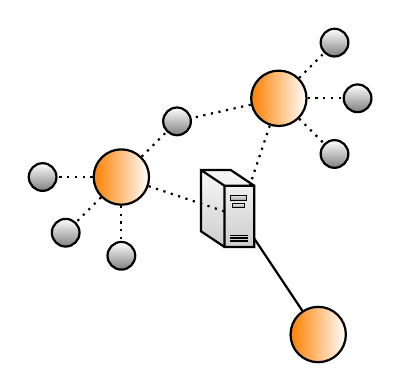
\begin{tikzpicture}[auto, thick]
      % Place super peers and connect them
      \foreach \place/\name in {{(0,-1)/a}, {(2,0)/b}, {(2.5, -3)/c}}
        \node[gateways] (\name) at \place {};
      \node[server] (d) at (1.5,-1.5) {};
      %
      \foreach \source/\dest in {a/d, b/d}
        \path[dotted] (\source) edge (\dest);
      \path (c) edge (d); % Non dotted
      %
      % Place normal peers
      \foreach \pos/\i in {above right of/1, right of/2, below right of/3}
        \node[motes, \pos =b ] (b\i) {};
      \foreach \speer/\peer in {b/b1,b/b2,b/b3}
        \path[dotted] (\speer) edge (\peer);
      %
      \foreach \pos/\i in {below left of/1, below of/2, left of/3, above right of/4}
        \node[motes, \pos =a ] (a\i) {};
      \foreach \speer/\peer in {a/a1,a/a2,a/a3,a/a4}
        \path[dotted] (\speer) edge (\peer);
      %
      \path[dotted] (b) edge (a4);
    \end{tikzpicture}
    \caption{Star topology\label{fig:startopology}}
\end{subfigure}
\hfill
\begin{subfigure}[b]{.5\textwidth}
    \centering
    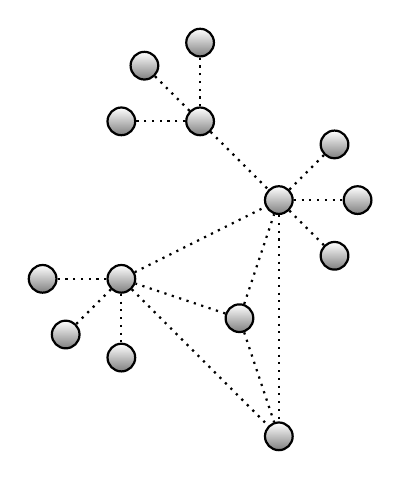
\begin{tikzpicture}[auto, thick]
      % Place super peers and connect them
      \foreach \place/\name in {{(0,-1)/a}, {(2,0)/b}, {(2, -3)/c}, {(1,1)/d}, {(1.5, -1.5)/f}}
        \node[motes] (\name) at \place {};
      \foreach \source/\dest in {a/b, a/c, b/c, d/b, f/a, f/b, f/c}
        \path[dotted] (\source) edge (\dest);
      %
      % Place normal peers
      \foreach \pos/\i in {above right of/1, right of/2, below right of/3}
        \node[motes, \pos =b ] (b\i) {};
      \foreach \speer/\peer in {b/b1,b/b2,b/b3}
        \path[dotted] (\speer) edge (\peer);
      %
      \foreach \pos/\i in {above left of/1, left of/2, above of/3}
        \node[motes, \pos =d ] (d\i) {};
      \foreach \speer/\peer in {d/d1,d/d2,d/d3}
        \path[dotted] (\speer) edge (\peer);
      %
      \foreach \pos/\i in {below left of/1, below of/2, left of/3}
        \node[motes, \pos =a ] (a\i) {};
      \foreach \speer/\peer in {a/a1,a/a2,a/a3}
        \path[dotted] (\speer) edge (\peer);
    \end{tikzpicture}
    \caption{Mesh Network Topology\label{fig:meshtopology}}
\end{subfigure}
\caption{Different LoRa Network Topologies\label{fig:topologies}}
\end{figure}





\section{Problem Statement}

The issue with \emph{LoRaWAN}, as studied
in~\cite{8030482}~\cite{10.1145/2988287.2989163} is its inability to scale
because of the addition of the following factors.

The first factor is channel sensing.
Detecting ongoing communication is impossible in LoRa because the \emph{Channel Activity Detection}
(CAD) feature can only detect the packet preamble.
This leads to unavoidable collision when a motes start its transmission
when another is already transmitting.
On collision, packets are retransmitted using a back-off strategy till the
message has been correctly received or the number of trials has reached its
maximum.
This implies a higher energy consumption for the motes and more radio
channel usage.
As the network gets denser~\cite{8030482}, the effect of collisions gets
increasingly significant with little to no packets received by gateways.

% TODO Figure from the paper about received packets ?

Second, the European sub-GHz ISM band has set a duty cycle of \emph{1\%} meaning that
each node and gateway can transmit \emph{36 sec/hour} maximum.
The duty cycle regulations in place for these ISM bands on every
transmitting device (motes and gateways) is also a limiting factor
for LoRaWAN (\cite{8030482}).

% TODO {Add some reference to ISM regulations}

Finally, Link quality also influences LoRaWAN's efficiency.
Environmental factors like temperature,
humidity~\cite{evaluation_of_the_reliability_of_lora}, and the topology of the
terrain~\cite{lorajambalaya}, influence the link quality.
All these factors make network coverage typically not uniform
as shown in Fig~\ref{fig:coverage}.
Motes on the border of the gateway coverage area may struggle to
achieve a full transmission.

Also, gateways could restrain the deployment of LoRa networks.
They might not be deployed everywhere as they require more demanding infrastructure
than battery-operated motes.
That is the case for the monitoring of pipelines and tunnels~\cite{Abrardo_2019},
for which one could prefer to only install motes running on batteries
which organise in a linear topology and can work without the help of gateways.
They can also be a single point of failure of the network when a single
gateway covers a portion of the network.

\begin{figure}[H]
    \centering
    \def\angle{0}
    \def\radius{3}
    \begin{tikzpicture}[nodes = {font=\sffamily}]
      \foreach \color in {
            yellow,
            red,
            yellow,
            white,
            red,
            yellow,
            white,
            yellow,
            white,
            white,
            red,
            red,
        } {
        \ifx\color\empty\else
            \draw[fill={\color!50},draw={\color}] (0,0) -- (\angle:\radius)
              arc (\angle:\angle+30:\radius) -- cycle;
            \pgfmathparse{\angle+30}
            \xdef\angle{\pgfmathresult}
        \fi
        };
        \xdef\radius{2.5}
        \foreach \color in {
            yellow,
            red,
            yellow,
            yellow,
            red,
            white,
            yellow,
            red,
            white,
            white,
            white,
            white,
        } {
        \ifx\color\empty\else
            \draw[fill={\color!50},draw={\color}] (0,0) -- (\angle:\radius)
              arc (\angle:\angle+30:\radius) -- cycle;
            \pgfmathparse{\angle+30}
            \xdef\angle{\pgfmathresult}
        \fi
        };
        \xdef\radius{2}
        \foreach \color in {
            yellow,
            red,
            green,
            red,
            yellow,
            white,
            yellow,
            white,
            white,
            white,
            white,
            white,
        } {
        \ifx\color\empty\else
            \draw[fill={\color!50},draw={\color}] (0,0) -- (\angle:\radius)
              arc (\angle:\angle+30:\radius) -- cycle;
            \pgfmathparse{\angle+30}
            \xdef\angle{\pgfmathresult}
        \fi
        };
        \xdef\radius{1.5}
        \foreach \color in {
            yellow,
            red,
            yellow,
            yellow,
            yellow,
            green,
            yellow,
            white,
            red,
            white,
            white,
            white,
        } {
        \ifx\color\empty\else
            \draw[fill={\color!50},draw={\color}] (0,0) -- (\angle:\radius)
              arc (\angle:\angle+30:\radius) -- cycle;
            \pgfmathparse{\angle+30}
            \xdef\angle{\pgfmathresult}
        \fi
        };
        \xdef\radius{1}
        \foreach \color in {
            green,
            green,
            green,
            yellow,
            yellow,
            yellow,
            white,
            white,
            yellow,
            red,
            yellow,
            red,
        } {
        \ifx\color\empty\else
            \draw[fill={\color!50},draw={\color}] (0,0) -- (\angle:\radius)
              arc (\angle:\angle+30:\radius) -- cycle;
            \pgfmathparse{\angle+30}
            \xdef\angle{\pgfmathresult}
        \fi
        };
        \xdef\radius{0.5}
        \foreach \color in {
            green,
            green,
            yellow,
            yellow,
            green,
            green,
            yellow,
            red,
            yellow,
            green,
            green,
            green,
        } {
        \ifx\color\empty\else
            \draw[fill={\color!50},draw={\color}] (0,0) -- (\angle:\radius)
              arc (\angle:\angle+30:\radius) -- cycle;
            \pgfmathparse{\angle+30}
            \xdef\angle{\pgfmathresult}
        \fi
        };
    \end{tikzpicture}
\caption{Typical gateway coverage\cite{lorajambalaya}\label{fig:coverage}}
\begin{tabular}{r@{: }l r@{: }l}

\begin{tikzpicture}\draw[fill=green,line width=1pt]  circle(1ex);\end{tikzpicture} & Good\ Connection & 
\begin{tikzpicture}\draw[fill=yellow,line width=1pt]  circle(1ex);\end{tikzpicture} & Intermediate\ Connection\\

\begin{tikzpicture}\draw[fill=red,line width=1pt]  circle(1ex);\end{tikzpicture} & Bad\ Connection & 
\begin{tikzpicture}\draw[fill=white,line width=1pt]  circle(1ex);\end{tikzpicture} & No\ Connection 
\end{tabular}
\end{figure}




Multi-hop networks, as represented in Fig~\ref{fig:meshtopology}, can be a solution to
the LoRaWAN scaling issues~\cite{8115756}.
Participants of the network do not directly send message to gateways, but
instead, pass messages to their neighboring nodes.
The use of a multi-hop routing protocol increases the reliability, the coverage
and allows to adapt to changes in the network (because of moving or failing nodes)
at the expense of higher energy consumption in the relaying motes.

Multi-hop routing protocols are de facto strong candidates for filling in the
routing tables for nodes deployed for large area monitoring
applications where gateways may be hard and costly to deploy and where blind
spots often arise.
This solution can potentially decrease the energy consumption of bordering
nodes that usually struggle to achieve successful communication in non-optimal
conditions.

\paragraph{}

Work to create a multi-hop routing protocol for LoRa multi-hop netowkrs has
already been done~\cite{8115756, DIAS2018424, 8856256, Abrardo_2019, duong2018},
but two main problems stand out from this similar work.

First, most studies consider that the motes are always-on and
neglect the problem of probable energy depletion.
LPWAN were designed to be used with battery operated motes that spend most of
his time sleeping and always-on motes go against that.
A solution to this first matter would be to use time-slotted channel access.
Synchronized nodes would be able to use a scheduling mechanism that tell them
when to wake-up to transmit or receive a packet.
This will put nodes in sleeping mode the rest of the time.
It also allows a deterministic access method to avoid collisions.

Second, these protocols only use a single channel.
This reduces network capacity and increases the risk of
interference.

\section{Approach}

Multi-hop routing solution already exists and can work on top of LoRa.
But until now LoRa multi-hop networks lacked a reliable and power efficient MAC protocol
to use in conjunction with routing protocols like the routing protocol for low power
and lossy networks (RPL).

The \emph{IEEE 802.15.4e} Time-Slotted Channel Hopping (TSCH) MAC protocol
has been designed for organizing reliable low power networks, we want to
investigate whether it would be a good candidate MAC protocol for LoRa based
multi-hop networks.
Using TSCH could actually solve many of the previous aforementioned issues.
First, TSCH uses channel hopping, making it resilient to external interference and
channel jamming and thus improving the reliability.
Second, TSCH uses synchronized motes and the notion of time slots to be able to organize
deterministic medium access, together with a schedule that will be designed to
minimize collisions and make the nodes sleep in slots in which no communication
need to take place.
An example of a schedule is Orchestra~\cite{duquennoy2015} that adapts to the
communication given by the routing protocol.
Adapting the TSCH protocol for LoRa would allow low power,
reliable and collision-free high-density networks, running over standards
multi-hop routing protocols.

\paragraph{}

This thesis aims to adapt the TSCH MAC protocol for LoRa.
thus bringing a reliable, long-range, and low power IPv6 multi-hop
solution to the LoRa ecosystem.

In order to achieve this, I will adapt the current TSCH implementation of
the Contiki operating system (OS) (originally developed for 802.15.4 compliant radio protocol)
to work with the longer delay induced by a low data-rate protocol like LoRa.
I will also implement a radio driver for the RN2483 in Contiki to have a
reliable LoRa radio driver working on the platform that I can adapt for my
needs.
In the end, I will have a fully working modified version of TSCH running on a
\emph{Zolertia RE-Mote} development board.

Testing my implementation in conjunction with RPL and the Orchestra schedule
for TSCH will successfully achieve multi-hop routing and thus demonstrating its
feasibility with LoRa.
An additional test ran over a jammed radio channel will show the reliability of
TSCH with LoRa.

\paragraph{}

Progress toward adapting TSCH for LoRa in~\cite{8847137} and~\cite{njomgang_2018},
has already been conducted in the previous year at \emph{VUB}.
This thesis builds on the combined efforts of previous work.

\section{Thesis Outline}

The next chapter will give the background information and context needed to
understand the building blocks to achieve my end goal.
It will also give an overview of the related work on the subject of
LoRa multi-hop communications.
Chapter \ref{section:radio} gives the implementation details of realising a driver for the
RN2483 in Contiki OS and the experimentation with the driver.
Chapter \ref{section:tsch} gives instructions and guidelines for adapting and
operating TSCH with LoRa on Contiki OS and reports on the different testing I conducted.
Chapter \ref{section:conclusion} will conclude the work by summarizing it and
will suggest possible futur research on the subject.


\chapter{Context}

% As of today little work has been done on creating a multihop LoRa Network (see Kris Paper on RPL LoRa in context section)

\section{LoRa}

\label{section:lora}

\paragraph{Packet Format}
\paragraph{Chirp Spread Spectrum (CSS) modulation}
\paragraph{Transmission Power}
\paragraph{Spreading Factor}

The higher the \emph{SF} the longer the communication range get while the
transmission also get slower. Frames can be sent at the same time if they are
all sent with a different spreading factors\cite{8030482}.

The data rate can range from 0.3kbps to 27kbps depending on the \emph{SF} % TODO Calculation needed

\paragraph{Bandwidth}
\paragraph{Coding-Rate}
\paragraph{Channels}

% See 'Understanding the limits of LoRaWAN' the 3 channels definition in Europe

\paragraph{Time On Air}

\begin{equation}
  \label{eq:tsym}
  T_{sym} = \frac{2^{SF}}{BW}
\end{equation}
\begin{equation}
  \label{eq:tpreamble}
  T_{preamble} = (n_{preamble} + 4.25)T_{sym}
\end{equation}
\begin{equation}
  \label{eq:payloadsymnb}
  payloadSymbNb = 8 + \max(ceil(\frac{8PL - 4SF + 28 + 16 - 20H}{4(SF - 2DE)})(CR + 4),0)
\end{equation}
\begin{equation}
  \label{eq:tpayload}
  T_{payload} = payloadSymNb T_{sym}
\end{equation}
\begin{equation}
  \label{eq:tpacket}
  T_{packet} = T_{preamble} + T_{paylaod}
\end{equation}

\section{TSCH}

TSCH is a MAC layer protocols designed for the low power and reliable
communications.
% And aims to achieve that 

\begin{description}
  \item[Channel Hopping] for a better usage of the band and less interference.
  \item[Time-division multiple access] or (TDMA) by assigning time-slots for each
    participant in the network avoiding collisions.
  \item[Synchronization] time-synchronized nodes syncing their clock with each
    other.
\end{description}

In the following section I will present the TSCH building blocks.

\subsection{Time Slots}

Time slots are a fixed unit of time to execute the TSCH network operations. 
The duration of the time slot is not standardized and depend on the physical 
layer we are using. 
Although, it has to be long enough for the longest frame size to be sent
between two nodes with an acknowledgement~\cite{rfc7554}. 
All time slots in a TSCH network have to be the same duration.

For each time slots operations, a schedule orchestrate what each
node of the network will use his time-slot for.

\begin{description}
  \item [Transmit] if a packet is on the outgoing buffer of the node.
  \item [Receive] listen for incoming packets that may arrive.
  \item [Sleep]
\end{description}

Because \emph{Channel Hopping} increase the network capacity a single time-slot
can be shared between multiple device to transmit at the same time on different
channels.

We can define \emph{links} as being made up of time slots and
channels~\cite{Chen2013PerformanceAO}.

\begin{equation}
  \label{eq:links}
  link = (TimeSlot_{number}, Channel_{offset})
\end{equation}

Multiple links constitute a time slot (dependent on the number of channel
available). Devices can transmit on different links during the same time slot.

\subsection{Slotframes}

Slotframes are a group of time slots that repeats over time as represented
in~\ref{fig:timeslots}. 

The size of the slotframe will directly impact on the energy consumption of
each node as increasing the size will decrease the number of time a node has
to exit sleep mode to listen or transmit packets.

\begin{figure}[H]
  \centering

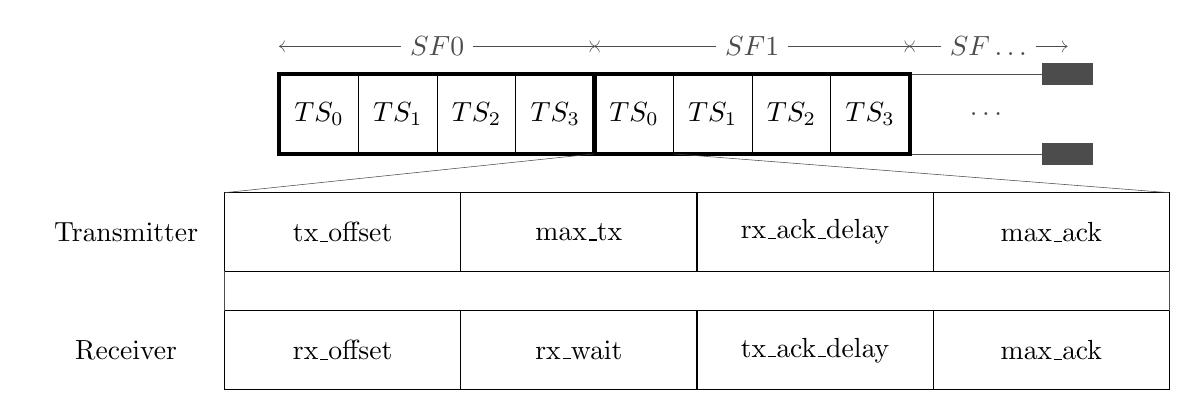
\begin{tikzpicture}[
  timeslot/.style={draw, rectangle, minimum size=1cm},
  description/.style={draw, rectangle, minimum size=1cm},
  arr/.style={help lines,black!70,<->},
]

\foreach [evaluate={\ts=int(mod(\i, 4))}] \i in {0,...,7} {
  \node (ts\i) [timeslot] at (\i, 0) {$TS_{\ts}$};
}
\node (ts8) [minimum height=1cm, minimum width=2cm, black!70] at (8.5, 0) {\ldots};

\draw[help lines, black!70]
  (ts8.north west) -- (ts8.north east) node[fill=white, black!70] {$\ldots$};
\draw[help lines, black!70]
  (ts8.south west) -- (ts8.south east) node[fill=white, black!70] {$\ldots$};

\draw[ultra thick] 
  (ts0.south west) rectangle (ts3.north east)
  (ts4.south west) rectangle (ts7.north east);

\draw[arr]
  ([yshift=10pt]ts0.north west) -- node[fill=white] {$SF0$} ([yshift=10pt]{ts3.north east});
\draw[arr]
  ([yshift=10pt]ts4.north west) -- node[fill=white] {$SF1$} ([yshift=10pt]{ts7.north east});
\draw[arr]
  ([yshift=10pt]ts8.north west) -- node[fill=white] {$SF\ldots$} ([yshift=10pt]{ts8.north east});

\begin{scope}[xshift=-1.2cm,yshift=-2cm,inner sep=0pt, outer sep=0pt]
  \node (desc) [fit={(-2.5,0) (0,1)}, label=center:{Transmitter}] {};
  \node (desc0) [description, fit={(0,0) (3,1)}, label=center:{tx\_offset}] {};
  \node (desc1) [description, fit={(3,0) (6,1)}, label=center:{max\_tx}] {};
  \node (desc2) [description, fit={(6,0) (9,1)}, label=center:{rx\_ack\_delay}] {};
  \node (desc3) [description, fit={(9,0) (12,1)}, label=center:{max\_ack}] {};
\end{scope}

\draw[help lines, black!70,-]
  ([yshift=0pt]ts4.south west) -- 
  ([yshift=0pt]{desc0.north west});
\draw[help lines, black!70,-]
  ([yshift=0pt]ts4.south east) -- 
  ([yshift=0pt]{desc3.north east});

\begin{scope}[xshift=-1.2cm,yshift=-3.5cm,inner sep=0pt, outer sep=0pt]
  \node (ddesc) [fit={(-2.5,0) (0,1)}, label=center:{Receiver}] {};
  \node (ddesc0) [description, fit={(0,0) (3,1)}, label=center:{rx\_offset}] {};
  \node (ddesc1) [description, fit={(3,0) (6,1)}, label=center:{rx\_wait}] {};
  \node (ddesc2) [description, fit={(6,0) (9,1)}, label=center:{tx\_ack\_delay}] {};
  \node (ddesc3) [description, fit={(9,0) (12,1)}, label=center:{max\_ack}] {};
\end{scope}

\draw[help lines, black!70,-]
  ([yshift=0pt]desc0.south west) -- 
  ([yshift=0pt]{ddesc0.north west});
\draw[help lines, black!70,-]
  ([yshift=0pt]desc3.south east) -- 
  ([yshift=0pt]{ddesc3.north east});

\end{tikzpicture}

\caption{Slotframes representation with the timings\label{fig:tstiming}}
\end{figure}


\subsection{Scheduling}

\subsection{Absolute Slot Number}

ASN is a shared counter between all the devices that define the number of time slots 
elapsed since the start of the start of the network.
It is increased after each time slot.

\subsection{Channel Hopping}

\subsection{Synchronization}

\paragraph{Cost of the Synchronization}

% * Nodes are required to synchronize their time source periodically
% * It's highly dependant on the clock quality

\section{6LoWPAN}

% 6TOP Sublayer

\section{Contiki OS}

\section{Related work}

\subsection{Time-Slotted LoRa}

\subsection{Multihop LoRa}




\chapter{Radio Driver for Zolertia with the RN2483 module}

% Most of the LoRaWAN features were not implemented or tested since this was out of the scope of this project.

Since the \emph{Zolertia RE-Mote REV-B} don't support \emph{LoRa} out of the
box we have to implement a software driver for the Microchip \emph{RN2483} LoRa
module.

\section{Preliminary work}

Last year \emph{Roald Van Glabbeek} started to work on the \emph{RN2483} module
in the course of his master thesis~\cite{8847137} aiming on doing further
research on \emph{energy efficient lora multihop networks}. For this purpose he
created a \emph{RN2483 Shield} adapted to the pin configuration of the
\emph{Zolertion RE-Mote REV-B} and started a driver implementation for the
Contiki-OS\@. The first part of my work consisted in implementing a reliable
and featurefull radio driver for the \emph{RN2483} module working in the last
version of \emph{contiki-ng}.

\section{RN2483 Module Structure}

Developped by \emph{Microchip} the \emph{RN2483} is a LoRa module working on
433 and 868Mhz band . The module is specically design to work with LoRaWAN
compliant network by including a set of commands specifically designed for
seamless connection with to a \emph{LoRaWAN} network. The module design is
aiming for ease of use over performance and low power.
All communication with the module are done with a \emph{UART} ASCII command
interface making it easy to interact with the module by a human that could be
entering command on a terminal and reading the response back in a human
readable format like in Fig~\ref{fig:pcconn}.

\begin{figure}[H] % TODO More info on axis
\centering
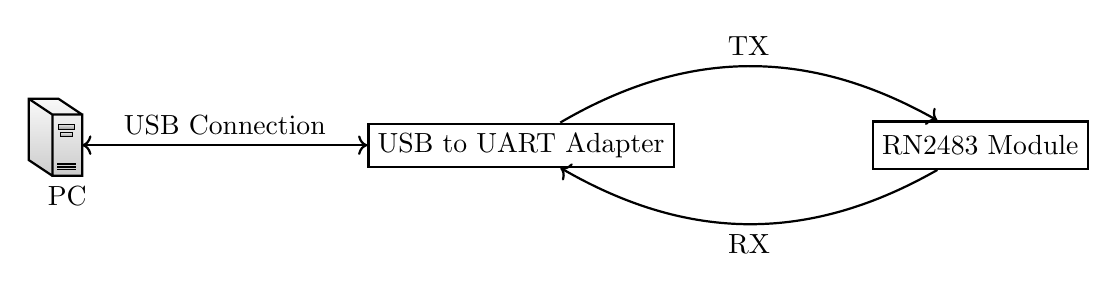
\begin{tikzpicture}[auto, thick]
  \node(pc) [server, label=below:{PC}] {};
  \node(ftdi) [draw, rectangle, right=of pc, right=4cm] {USB to UART Adapter};
  \node(module) [draw, rectangle, minimum size=6mm, right=of ftdi, right=2.5cm] (module) {RN2483 Module};

  \path (pc) edge[<->] node[]{USB Connection} (ftdi) ;
  \path (ftdi) edge[->,bend left] node[text width=1cm, align=center]{TX} (module);
  \path (module) edge[->,bend left] node[text width=1cm, align=center]{RX} (ftdi);
\end{tikzpicture}
\caption{Simple communication with the module scenario}
\label{fig:pcconn}
\end{figure}


% Command type division
The module's interface include three types of cammands that enable access to
different functions.

\begin{itemize}
  \item \emph{mac} for the LoRaWAN configurations and control.
  \item \emph{radio} for the low-level radio commands to access the transceiver
    directly without the LoRaWAN interface.
  \item \emph{sys} for the module specific configurations such as the module
    GPIOs state, \emph{sleep}, EEPROM memory access, \ldots
\end{itemize}

\section{Testing Setup}

My testing setup was the same as~\cite{8847137}, I used a Zolertia RE-Mote
Rev-B dev board connected to a RN2483 breakout board and connected them like in
Fig~\ref{fig:schemaconn}.

\begin{figure}[H]
  \centering
  \includegraphics[scale=0.75]{thesis.tex/chapters/driver/fig/conn_diag.pdf}
  \caption{Hardware connection}
  \label{fig:schemaconn}
\end{figure}

\section{Implementation}

\subsection{Structure}

\subsection{Synchronous communication}

\subsection{Contiki Radio Driver}

\section{Validation test}


\chapter{Time-Slotted Channel Hopping Implementation for LoRa\label{section:tsch}}

\section{Porting TSCH}

\subsection{Channels}

\subsection{Timestamp}

\subsection{Radio delay}

\subsection{$\mu s$ and rtimer ticks conversion}

\subsection{LoRa Time On Air}

\section{Adaptation of the timing}

\paragraph{Timing size issue}

\section{Testing}

\section{Considerations}


\chapter{Conclusion and further work\label{section:conclusion}}

The goal of the thesis was to adapt TSCH to work with LoRa to achieve power
efficient and reliable multihop networking with LoRa on Contiki OS with the 
RN2483 LoRa module.

\paragraph{}

My work was divided into two parts. 
In the first part, I successfully implemented a working driver for the RN2483
module. 
Section~\ref{section:pingpong} detail how I ran a ping pong
example based on that driver to prove the driver is fully working with the
rest of the applications.

The second part should have been on paper limited to the adaptations of the
timing variable of the TSCH protocol to work with LoRa.
In the end, the long delay induced by LoRa communication turned out to 
not work seamlessly with Contiki. 
The second part of my work became a bug hunt with the TSCH implementation 
I detailed in section~\ref{section:timingparameters}.
The TSCH parameters I used were used as a mean to achieve a working version of
the protocol rather than getting the optimal version of TSCH with LoRa.
I finally managed to make LoRa work with TSCH in section~\ref{section:tschtesting} by
demonstrating my work integrates into the 6TiSCH networking stack.
I addressed my concerns about the reliability of my implementation
because of the drift issues caused by the hardware in~\ref{section:driftissues}.

\paragraph{}

In his last year's master thesis, Roald Van Glabbeek suggested further research
should conduct a power analysis on the RN2483 module.
I responded to this statement in~\ref{section:energyconsumption} about how
achieving a low power network with TSCH and this module is impossible because
of the design of the module.

The good news is I'm confident that achieving a low power multi-hop network with 
a radio module like the SX1272 is possible.
This thesis explained what it takes to adapt TSCH for a new LoRa radio
module and the possible re-implementation of this project on a new radio module 
will then be facilitated. 

This would create a stable testing device that would allow us to measure meaningful 
data for the analysis of power consumption and reliability of the network.
The following tasks could be conducted

\begin{itemize}
  \item Determining the optimal TSCH parameters for LoRa. 
  \item Finding the optimal period between EB packets to keep a balance between
    low power usage and maintaining synchronization.
  \item Compare how it performs in regards to LoRaWAN. Is the TSCH overhead
    worth it ?
  \item The network capacity and transmission delay.
\end{itemize}

\paragraph{}

The ideal implementation would adapt its SF depending on the distance
between two hops.
In my implementation even though the different SF are supported, only operates
on a single SF at the time. 
We miss a lot of LoRa features with the single SF, supporting multiple SF at
the same time would increase the network throughput and increase the
transmission range for nodes with low reception.
The literature does not talk about using adaptive SF in a multi-hops
network except for~\cite{8115756} that could give us indications on the future
work on the subject.

\paragraph{}

Related work reinvented the wheel by implementing their multi-hop solution
using their own MAC protocol on top of LoRa.
Using TSCH, an already well studied MAC protocol,
and prooving it can work with the existing multi-hop routing solutions,
represents a step forward in the LoRa multi-hop networking research.
Reliable implementation, performance, and energy consumption tests, as well as 
using every SF to use the full LoRa capacity is the future challenge of the
subject.

\newpage

\printbibliography

\newpage

\begin{appendices}
\chapter{Table}

\section{LoRa}


\begin{table}[h!]
\centering
\begin{tabular}{@{}lll@{}}
\toprule
BW (kHz) & SF & bit rate (bits/sec) \\ \midrule
125     & 7 & 6836 \\
125     & 8 & 3906 \\
125     & 9 & 2197 \\
125     & 10 & 1220 \\
125     & 11 & 671 \\
125     & 12 & 366 \\
250     & 7 & 13671 \\
250     & 8 & 7812 \\
250     & 9 & 4394 \\
250     & 10 & 2441 \\
250     & 11 & 1342 \\
250     & 12 & 732 \\ \bottomrule
\end{tabular}
\caption{Bit rates depending on BW, and SF\label{table:bitrate}}
\end{table}


\begin{table}[h!]
\centering
\begin{tabular}{@{}lllll@{}}
\toprule
CR & BW (kHz) & SF7 (bits/sec) & SF8 (bits/sec) & SF10 (bits/sec) \\ \midrule
\multirow{2}{*}{$\frac{4}{5}$} & 125000   & 5469           & 3125           & 976             \\
  & 250000   & 10937          & 6250           & 1953            \\
\multirow{2}{*}{$\frac{4}{6}$} & 125000   & 4557           & 2604           & 813             \\
  & 250000   & 9114           & 5208           & 1627            \\
\multirow{2}{*}{$\frac{4}{8}$} & 125000   & 3417           & 1954           & 660             \\
  & 250000   & 6835           & 3906           & 1220            \\ \bottomrule
\end{tabular}
\caption{Data rates depending on CR, BW, and SF\label{table:datarate}}
\end{table}

\section{RN2483 Timing Measurements and Predictions}

\begin{table}[H]
\centering
\begin{tabular}{|l|l|l|}
\hline
\rowcolor[HTML]{C0C0C0}
  \multicolumn{1}{|c|}{\cellcolor[HTML]{C0C0C0}Bytes} & Time ($\mu s$) & Prediction ($\mu s$) \\ \hline
1                                                   & 3080      & 3021       \\ \hline
4                                                   & 3560      & 3528       \\ \hline
8                                                   & 4200      & 4204       \\ \hline
16                                                  & 5550      & 5556       \\ \hline
32                                                  & 8280      & 8260       \\ \hline
64                                                  & 13680     & 13668      \\ \hline
110                                                 & 21430     & 21442      \\ \hline
\end{tabular}
\caption{Transmission Time\label{table:measurementtx}}
\end{table}

\begin{table}[H]
\centering
\begin{tabular}{|l|l|l|}
\hline
\rowcolor[HTML]{C0C0C0}
\multicolumn{1}{|c|}{\cellcolor[HTML]{C0C0C0}Bytes} & Time ($\mu s$) & Prediction ($\mu s$) \\ \hline
1                                                   & 820       & 898        \\ \hline
4                                                   & 2350      & 2332       \\ \hline
8                                                   & 4240      & 4244       \\ \hline
16                                                  & 8160      & 8068       \\ \hline
32                                                  & 15600     & 15716      \\ \hline
64                                                  & 31100     & 31012      \\ \hline
110                                                 & 53200     & 53000      \\ \hline
\end{tabular}
\caption{Reception Spreading Factor 7\label{table:rxsf7}}
\end{table}

\begin{table}[H]
\centering
\begin{tabular}{|l|l|l|}
\hline
\rowcolor[HTML]{C0C0C0}
\multicolumn{1}{|c|}{\cellcolor[HTML]{C0C0C0}Bytes} & Time ($\mu s$) & Prediction ($\mu s$) \\ \hline
1                                                   & 1500      & 1529       \\ \hline
4                                                   & 3240      & 2963       \\ \hline
8                                                   & 5060      & 4875       \\ \hline
16                                                  & 8840      & 8699       \\ \hline
32                                                  & 16700     & 16347      \\ \hline
64                                                  & 31700     & 31643      \\ \hline
110                                                 & 53300     & 53631      \\ \hline
\end{tabular}
\caption{Reception Spreading Factor 8\label{table:rxsf8}}
\end{table}

\begin{table}[H]
\centering
\begin{tabular}{|l|l|l|}
\hline
\rowcolor[HTML]{C0C0C0}
\multicolumn{1}{|c|}{\cellcolor[HTML]{C0C0C0}Bytes} & Time ($\mu s$) & Prediction ($\mu s$) \\ \hline
1                                                   & 3160      & 3287       \\ \hline
4                                                   & 4560      & 4721       \\ \hline
8                                                   & 6500      & 6633       \\ \hline
16                                                  & 10120     & 10457      \\ \hline
32                                                  & 17900     & 18105      \\ \hline
64                                                  & 33200     & 33401      \\ \hline
110                                                 & 55200     & 55389      \\ \hline
\end{tabular}
\caption{Reception Spreading Factor 9\label{table:rxsf9}}
\end{table}

\begin{table}[H]
\centering
\begin{tabular}{|l|l|l|}
\hline
\rowcolor[HTML]{C0C0C0}
\multicolumn{1}{|c|}{\cellcolor[HTML]{C0C0C0}Bytes} & Time ($\mu s$) & Prediction ($\mu s$) \\ \hline
1                                                   & 6100      & 6235       \\ \hline
4                                                   & 7400      & 7669       \\ \hline
8                                                   & 9660      & 9581       \\ \hline
16                                                  & 13560     & 13405      \\ \hline
32                                                  & 21040     & 21053      \\ \hline
64                                                  & 36400     & 36349      \\ \hline
110                                                 & 58400     & 58337      \\ \hline
\end{tabular}
\caption{Reception Spreading Factor 10\label{table:rxsf10}}
\end{table}

\chapter{Listing}

\section{Packet timestamp implementation\label{code:timestampimpl}}

\begin{lstlisting}[language=c]
static radio_result_t
rn2483_get_object(radio_param_t param, void *dest, size_t size)
{
  switch(param) {
  case RADIO_PARAM_LAST_PACKET_TIMESTAMP:
    if(size != sizeof(rtimer_clock_t) || !dest) {
      return RADIO_RESULT_INVALID_VALUE;
    }
    *(rtimer_clock_t *)dest = RN2483_DEV.packet_timestamp
      - US_TO_RTIMERTICKS_64(
          RX_RECEIVING_DELAY_US(RN2483_DEV.rx_len)
          + t_packet(&(RN2483_DEV.radio), RN2483_DEV.rx_len)
          + TRANSMISSION_TIME_US(RX_CMD_LENGTH(RN2483_DEV.rx_len))
      );
    return RADIO_RESULT_OK;
  }
}
\end{lstlisting}



\section{Custom Schedule Code\label{code:customsched}}

\begin{lstlisting}
static linkaddr_t node_1_address = {{
  0x00, 0x12, 0x4b, 0x00, 0x14, 0xd5, 0x2f, 0x2a
}};
static linkaddr_t node_2_address = {{
  0x00, 0x12, 0x4b, 0x00, 0x14, 0xd5, 0x2d, 0xac
}};
static linkaddr_t node_3_address = {{
  0x00, 0x12, 0x4b, 0x00, 0x14, 0xd5, 0x2d, 0xbc
}};
static linkaddr_t node_4_address = {{
  0x00, 0x12, 0x4b, 0x00, 0x14, 0xd5, 0x2f, 0x09
}};

void
tsch_schedule_custom(void)
{
  struct tsch_slotframe *sf_custom;
  tsch_schedule_remove_all_slotframes();
  sf_custom = tsch_schedule_add_slotframe(0, TSCH_SCHEDULE_DEFAULT_LENGTH);
  tsch_schedule_add_link(sf_custom,
      LINK_OPTION_RX | LINK_OPTION_TX | LINK_OPTION_SHARED | LINK_OPTION_TIME_KEEPING,
      LINK_TYPE_ADVERTISING, &tsch_broadcast_address,
      0, 0);

  if (linkaddr_node_addr.u8[7] == node_1_address.u8[7]) {
    tsch_schedule_add_link(sf_custom, LINK_OPTION_RX, LINK_TYPE_NORMAL, &node_2_address, 1, 0);
    tsch_schedule_add_link(sf_custom, LINK_OPTION_RX, LINK_TYPE_NORMAL, &node_3_address, 2, 0);
    tsch_schedule_add_link(sf_custom, LINK_OPTION_TX, LINK_TYPE_NORMAL, &node_3_address, 4, 0);
  } else if (linkaddr_node_addr.u8[7] == node_2_address.u8[7]) {
    tsch_schedule_add_link(sf_custom, LINK_OPTION_TX, LINK_TYPE_NORMAL, &node_1_address, 1, 0);
    tsch_schedule_add_link(sf_custom, LINK_OPTION_RX, LINK_TYPE_NORMAL, &node_3_address, 3, 0);
    tsch_schedule_add_link(sf_custom, LINK_OPTION_RX, LINK_TYPE_NORMAL, &node_4_address, 5, 0);
    tsch_schedule_add_link(sf_custom, LINK_OPTION_TX, LINK_TYPE_NORMAL, &node_4_address, 6, 0);
  } else if (linkaddr_node_addr.u8[7] == node_3_address.u8[7]) {
    tsch_schedule_add_link(sf_custom, LINK_OPTION_TX, LINK_TYPE_NORMAL, &node_1_address, 2, 0);
    tsch_schedule_add_link(sf_custom, LINK_OPTION_TX, LINK_TYPE_NORMAL, &node_2_address, 3, 0);
    tsch_schedule_add_link(sf_custom, LINK_OPTION_RX, LINK_TYPE_NORMAL, &node_1_address, 4, 0);
  } else if (linkaddr_node_addr.u8[7] == node_4_address.u8[7]) {
    tsch_schedule_add_link(sf_custom, LINK_OPTION_TX, LINK_TYPE_NORMAL, &node_2_address, 5, 0);
    tsch_schedule_add_link(sf_custom, LINK_OPTION_RX, LINK_TYPE_NORMAL, &node_2_address, 6, 0);
  }
}
\end{lstlisting}

\end{appendices}

\end{document}

